%%%%%%%%
% Auteur : Jonathan Barnoud <jonathan@barnoud.net>
% Ce document est mis à disposition selon les termes de la licence
% Creative Commons Attribution 3.0 non transposée
% http://creativecommons.org/licences/by/3.O/
%%%%%%%%


\documentclass[xcolor=pdftex,dvipsnames,table,handout]{beamer}

%\setbeameroption{show notes}

\usepackage[utf8]{inputenc}
\usepackage[T1]{fontenc}
\usepackage[french]{babel}
\usepackage{xspace}

\usepackage{url}

\usepackage{pifont}
\usepackage{wasysym}

\usepackage{array}

\usepackage{palatino}

\usepackage{listings}

\usepackage{tikz}

\title{Conventions de style en python}
%\subtitle{M1 ISDD -- Projet de programmation Python}
\author{Jonathan Barnoud \url{jonathan.barnoud@univ-paris-diderot.fr}}
%\date{21 février 2012}
%\date{2012}
\date{}

\usetheme{jo}
%\usetheme{Warsaw}

% Define a HUGE font size
\makeatletter
\newcommand\HUGE{\@setfontsize\Huge{100}{85}}
\makeatother

\newcommand{\publi}[1]{{\footnotesize (#1)}}
\newcommand{\etal}{\textit{et al.}}

\renewcommand{\emph}[1]{\textbf{#1}}

\newenvironment{bigitem}{%
\begin{center}
\begin{minipage}{0.5\linewidth}
\Large%
\begin{itemize}}{%
\end{itemize}%
\end{minipage}
\end{center}}

\newenvironment{changemargin}[2]{%
  \begin{list}{}{%
    \setlength{\topsep}{0pt}%
    \setlength{\leftmargin}{#1}%
    \setlength{\rightmargin}{#2}%
    \setlength{\listparindent}{\parindent}%
    \setlength{\itemindent}{\parindent}%
    \setlength{\parsep}{\parskip}%
  }%
  \item[]}{\end{list}} 

\lstset{% paramètres du paquet listings
language={Python}, % no programming language
keywords={},
basicstyle=\ttfamily\bfseries, % affichage en petit du code
aboveskip=0.5\smallskipamount, % espace avant le listing
extendedchars=false, % allow utf-8
showstringspaces=false,
keywordstyle=\color{green},
}

\begin{document}
\titleframe{}

\section*{Introduction}

\begin{frame}{Pourquoi ?}
\begin{center}
\Huge{Améliorer la lisibilité}
\end{center}
\end{frame}

\begin{frame}{Convention ?}
\begin{center}
\Huge{Cohérence}
\vspace{1cm}

\Large{\only<2->{module}\only<3->{ > projet}\only<4->{ > équipe}\only<5->{ > langage}}
\end{center}
\end{frame}

\begin{frame}{Document de référence}
\begin{center}
\Huge{PEP 8}
\vspace{1cm}

\Large{\textit{Python Enhancement Proposal}}
\end{center}
\end{frame}


\begin{frame}{Plan}
\tableofcontents
\end{frame}

\section{Organisation du code}

\begin{frame}{Indentation}
\begin{center}
\Large{Espaces ou tabulations}
\vspace{2cm}

\Large{Pas de mélange}
\end{center}
\end{frame}

\begin{frame}{Indentation}
\begin{center}
\Huge{4 espaces}
\end{center}
\end{frame}

\begin{frame}{Indentation}{Configurer l'éditeur}
\begin{center}
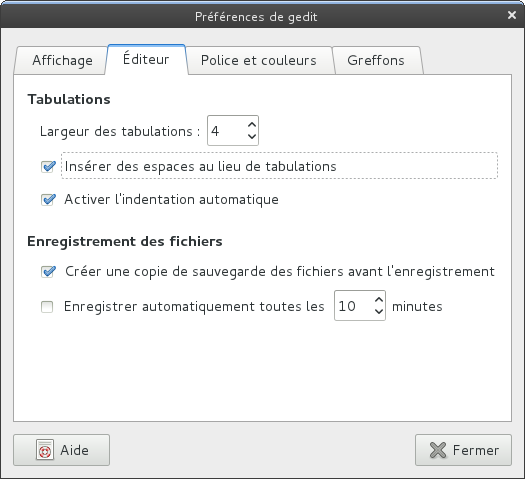
\includegraphics[width=0.7\linewidth]{img/Capture-Preferences-de-gedit}
\end{center}
\end{frame}

\begin{frame}{Taille d'une ligne}
\begin{center}
\Huge{Pas de lignes trop longues}
\end{center}
\end{frame}

\begin{frame}{Taille d'une ligne}
\begin{center}
\Huge{79 caractères}
\end{center}
\end{frame}

\begin{frame}{Taille d'une ligne}
\begin{center}
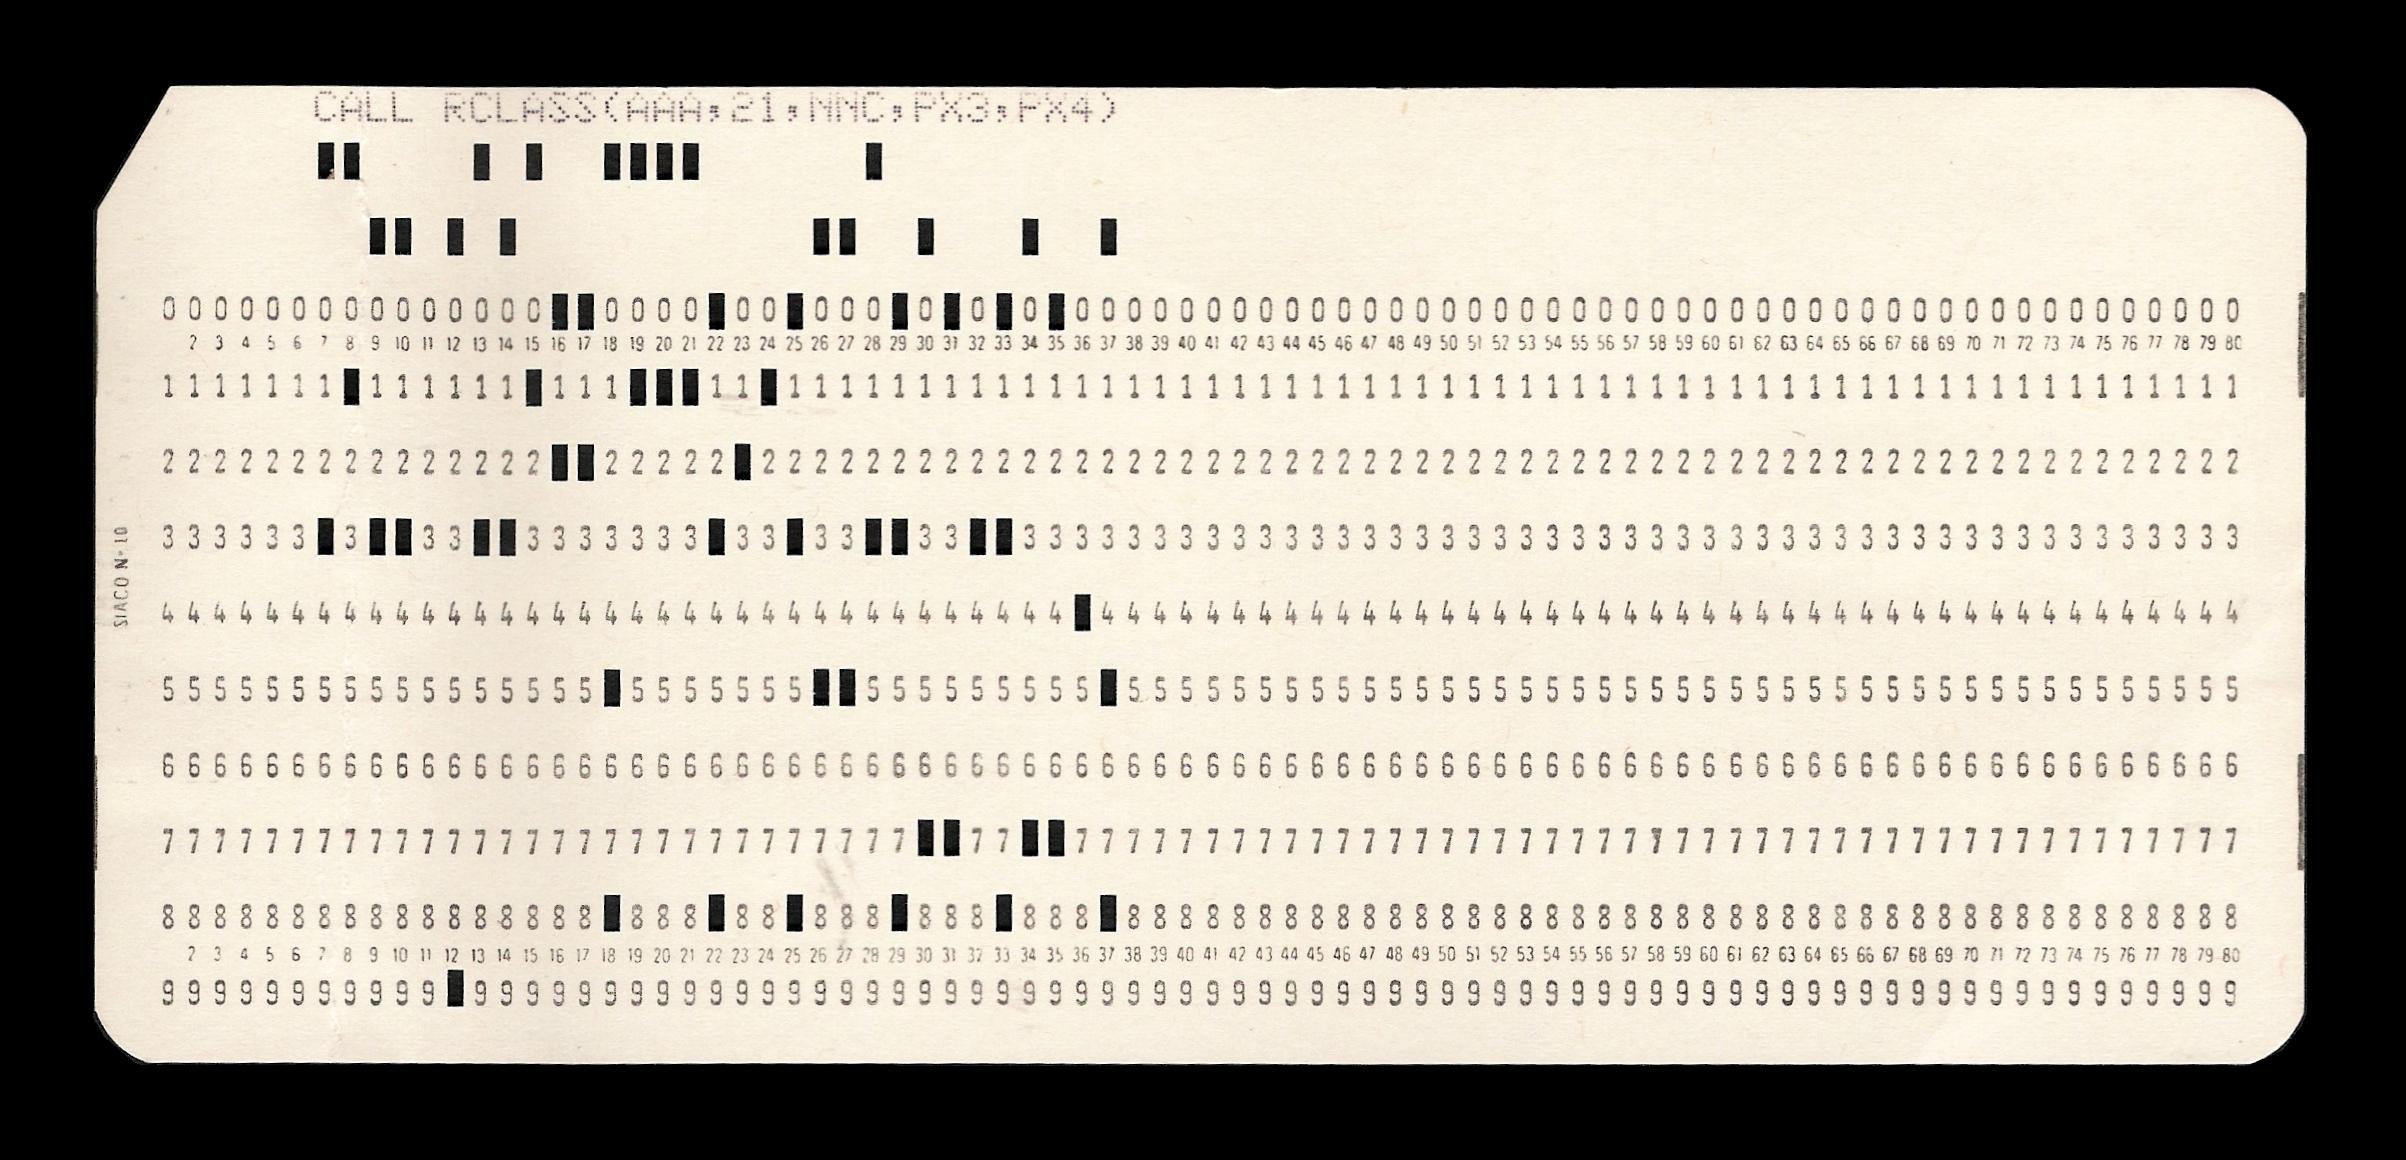
\includegraphics[width=0.9\linewidth]{img/Punched_card}
\end{center}
\hfill \footnotesize{Crédits : Mutatis mutandis, Creative commons by, \url{http://commons.wikimedia.org/wiki/File:Punched\_card.jpg}}
\end{frame}

\begin{frame}{Taille d'une ligne}
\begin{center}
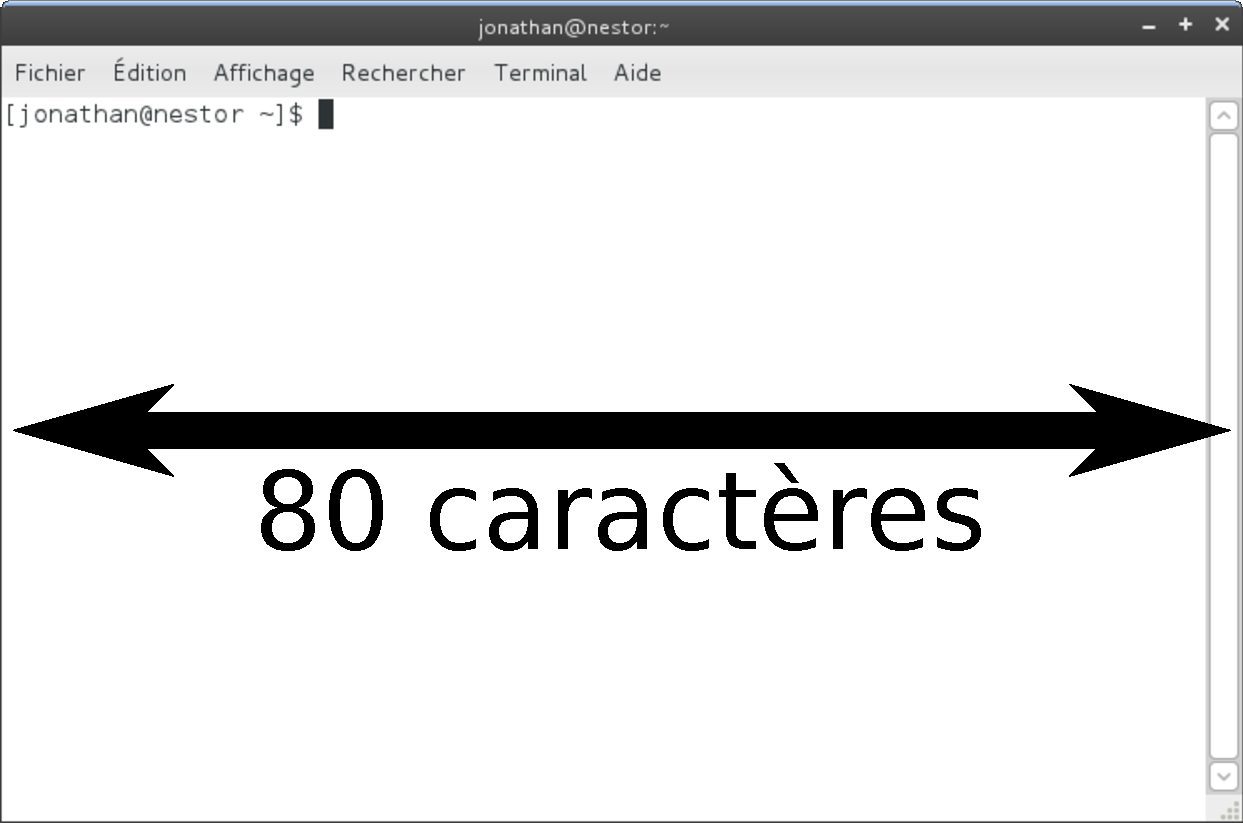
\includegraphics[width=0.7\linewidth]{img/Capture-Terminal.pdf}
\end{center}
\end{frame}

\begin{frame}[fragile]
\frametitle{Taille d'une ligne}
\begin{lstlisting}
morpion = [["X", "X", "O"],
           ["O", "X", "X"],
           ["X", "O", "O"]]

atome = {"type" : " CA ",
         "aa" : "Lys",
         "residu" : 43,
         "coordonnees" : (43.5, 67.8, 12.9),
        }
\end{lstlisting}
\end{frame}

\begin{frame}[fragile]
\frametitle{Taille d'une ligne}
\begin{lstlisting}
>>> print ("ATTCGCTAATCGATGC"
...        "GTCCCTAGGTTCCCGTAC"
...        "GGTCATCATCA"
...       )
ATTCGCTAATCGATGCGTCCCTAGGTTCCCGTACGGTCATCATCA
\end{lstlisting}
\end{frame}

\begin{frame}[fragile]
\frametitle{Taille d'une ligne}
\begin{lstlisting}
if (  -87 < phi < -27  and 
      -77 < psi < -17 ) :
    print "helix"

if -87 < phi < -27 and \
   -77 < psi < -17 :
    print "helix"
\end{lstlisting}
\end{frame}

\begin{frame}{Sauts de lignes}
\begin{itemize}
    \item Constitue des blocs visuels dans le code
    \item \textbf{2} saut de ligne entre deux définitions de fonctions ou de classes
    \item \textbf{1} sauts de ligne entre deux définitions de méthodes
\end{itemize}
\end{frame}

\section{Commentaires}

\begin{frame}[fragile]
\frametitle{Commentaires}
\begin{lstlisting}
# Un commentaire sur une ligne
\end{lstlisting}
\begin{lstlisting}
# Un commentaire un peu plus long
# sur deux lignes
\end{lstlisting}
\end{frame}

\begin{frame}[fragile]
\frametitle{\textit{Docstrings}}
\begin{lstlisting}
>>> def hello_world(name) :
...     """
...     Souhaite le bonjour à quelqu'un.
...     """
...     print "Hello %s" % name
... 
>>> help(hello_world)
Help on function hello_world in module __main__:

hello_world(name)
    Souhaite le bonjour à quelqu'un.
\end{lstlisting}
\end{frame}

%\begin{frame}[fragile]
%\frametitle{\textit{Docstrings}}
%\begin{lstlisting}
%def toto() :
%    """
%    Une docstring.
%
%    Sur plusieurs lignes.
%    """
%    return None
%
%def toto() :
%    """Une docstring.
%
%    Sur plusieurs lignes.
%    """
%    return None
%
%\end{lstlisting}
%\end{frame}

\begin{frame}[fragile]
\frametitle{\textit{Docstrings}}
\begin{itemize}
\item Pour les classes%
\begin{lstlisting}
class MaClasse :
    """
    Une classe qui fait pleins de trucs.
    """
\end{lstlisting}
\item Pour les modules%
\begin{lstlisting}
#!/usr/bin/env python
#-*- coding:utf-8 -*-

"""
Un super module !
"""
\end{lstlisting}
\end{itemize}
\end{frame}

\begin{frame}{\textit{Docstrings}}
\begin{itemize}
\item Qu'est-ce que ça fait ?
\item Pourquoi ça le fait ?
\item D'où ça vient ?
\item \textbf{Quels arguments ?}
\item \textbf{Quels retours ?}
\item Quels exceptions ?
\item Comment ça s'utilise ?
\end{itemize}
\end{frame}

\begin{frame}[fragile]
\frametitle{\textit{Doctests}}
\begin{lstlisting}
def somme(a, b) :
    """
    Calcul la somme de a et b.
    
    >>> somme(2, 3)
    5
    """
    return a + b
\end{lstlisting}
\begin{lstlisting}
import doctest
doctest.testmod()
\end{lstlisting}
\end{frame}

\begin{frame}{Sphinx}
\begin{center}
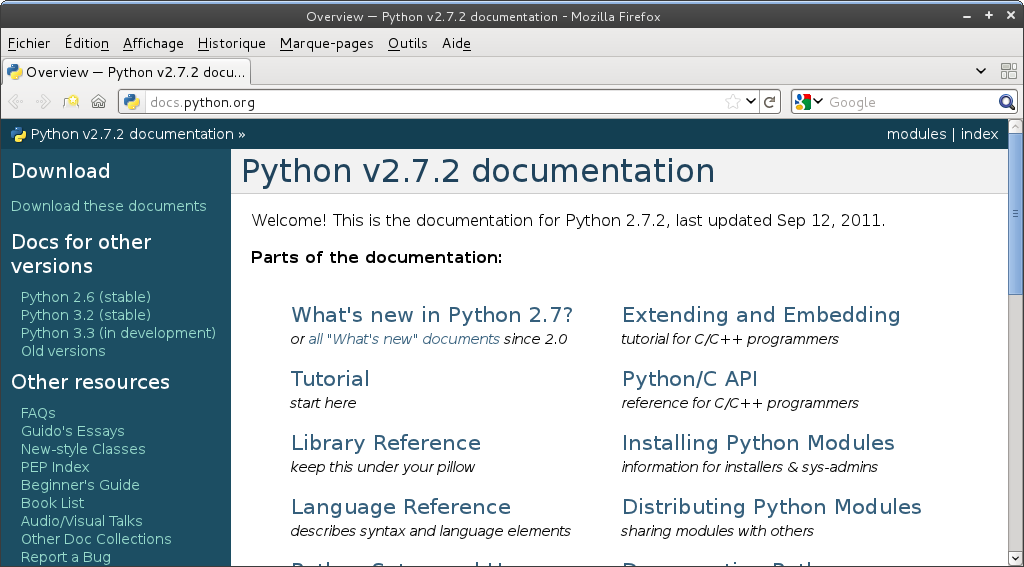
\includegraphics[width=\linewidth]{img/Capture-Python}
\end{center}
\end{frame}

\begin{frame}[fragile]
\protect{\tiny%
\begin{lstlisting}
    def check_go(self, direction) :
        """
        Check if it is possible to go in the given direction.

        :Parameters:
            - direction (string): can be "NORTH", "SOUTH", "EAST" or "WEST"

        :Exception:
            - OutOfMap : is raised if the coordinates are out of the map
            - BadCell : is raised if the given cell can't receive the item
            - ChrIncapacity : is raised if the character is not able to move
                this way because he have not enough action points, because
                he's dead or because of anything linked to the character himself
            - NoMap : is raised if the character is not on a map

        :Returns:
            The cost of the move in action points.
        """

\end{lstlisting}%
}
\end{frame}

\begin{frame}{Sphinx}
\begin{center}
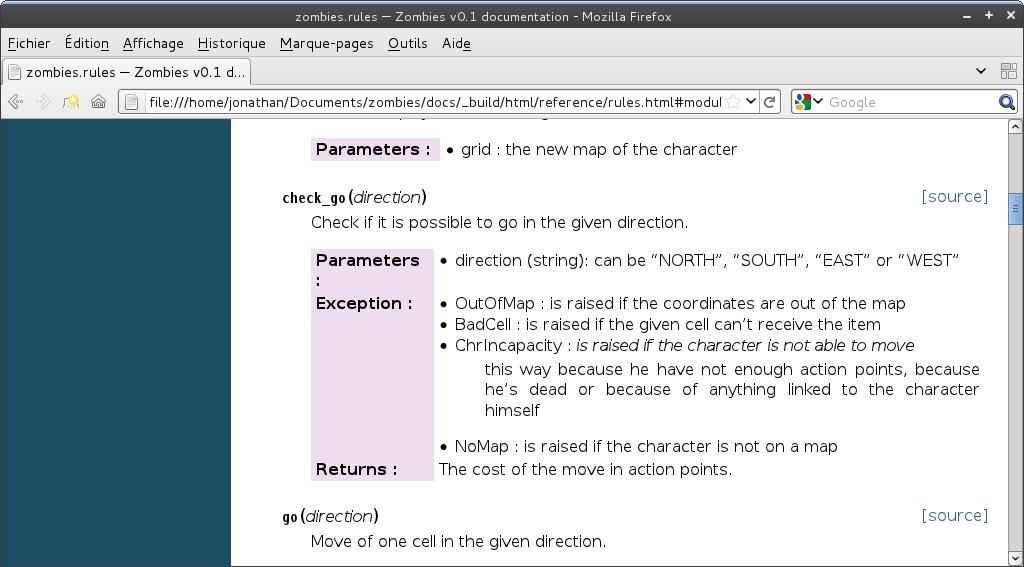
\includegraphics[width=\linewidth]{img/Capture-Sphinx}
\end{center}
\end{frame}

\begin{frame}{Sphinx}
\begin{center}
\Large{\url{http://sphinx-doc.org}}
\end{center}
\end{frame}

\section{Noms de variables}

\begin{frame}{Choix d'un nom de variable}
\begin{center}
\Huge{Noms explicites}
\end{center}
\end{frame}

\begin{frame}{Conventions de nommage}
\begin{itemize}
    \item variables et fonctions : \texttt{ma\_variable}
    \item constantes : \texttt{MA\_CONSTANTE}
    \item classes : \texttt{MaClasse}
    \item exeptions : \texttt{MyError}
\end{itemize}
\end{frame}

\section{Références}

\begin{frame}{Évaluer la qualité}
\begin{center}
\Large{\texttt{pylint mon\_script.py}}

\Large{\texttt{flake8 mon\_script.py}}
\end{center}
\end{frame}

\begin{frame}{Références}
\begin{center}

\includegraphics[width=0.5\linewidth]{img/pp}
\end{center}
\end{frame}

\begin{frame}{Références}
\begin{description}
    \item[PEP 8] \url{http://www.python.org/dev/peps/pep-0008/}
    \item[Bonnes pratiques] \url{http://bit.ly/OUkymD}
    %\url{https://larlet.fr/david/biologeek/archives/20080511-bonnes-pratiques-et-astuces-python/}
    \item[Sphinx] \url{http://sphinx-doc.org}
    \item[pylint] \url{http://www.logilab.org/857}
    \item[flake8] \url{http://flake8.readthedocs.org}
\end{description}
\end{frame}

\begin{frame}{Conclusion}
\begin{center}
    \Huge{import this}
\end{center}
\end{frame}

\begin{frame}[plain]
\vfill
\begin{center}
{\Large%
\url{github.com/jbarnoud/Cours-python}%
}
\vfill
\vfill
\vfill
{\tiny%

\includegraphics[width=1.5cm]{img/logo/cc_by}

Ce document est mis à disposition selon les termes de la licence Creative Commons Attribution 3.0 non transposée\newline
\url{http://creativecommons.org/licences/by/3.O/}
}
\end{center}
\end{frame}

\end{document}
